\newcommand{\partition}[1]{  


  \draw[thin]  (-0.5,-0.8) rectangle (2,3) node[right,xshift=-1cm,littletext]{Partition$_#1$};

  \draw[dashed, thin] (-0.5,2.7) node[right=0.2cm,littletext] {P-FP domain} -- +(2.5,0);

  \node[below] (F1)  at (0.8,2.50)  {\tiny (task*) scheduled};
  \node[below, xshift=-0.20cm] (F2)  at (0.8,2.20)  {\tiny (int) cpu};
  \node[below, xshift= 0.05cm] (F3)  at (0.8,1.90)  {\tiny (queue*) ready\_queue};
  \node[below, xshift=-0.45cm] (F4)  at (0.8,1.60)  {\tiny (spinlock) {lock}};
  \node[below, xshift=-0.20cm] (F5)  at (0.8,1.30)  {\tiny (sem*) mrsp};

  \draw[dashed, thin] (-0.5,0.7) node[right=0.2cm,littletext] {Local ceiling} -- +(2.5,0);

  \node[below] (F)  at (0.8,0.55)  {\tiny (int) {\color{red}ceiling}};

  \draw[dashed, thin] (-0.5,0) -- +(2.5,0);

  \node[below] (P)  at (0.75,-0.2)  {\footnotesize plugin interface};  

}


\newcommand{\mrsp}{

  \draw[thin]  (-0.5,-0.8) rectangle (2,2) node[right,xshift=-1.5cm,littletext]{Global resourse};

  \draw[dashed, thin] (-0.5,1.7) node[right=0.2cm,littletext] {MrsP} -- +(2.5,0);

  \node[below] (F1)  at (0.8,1.6)  {\tiny (task*) lock holder};
  \node[below, xshift=-0.1cm] (F2)  at (0.8,1.3)  {\tiny (int*) ceilings};
  \node[below, xshift=-0.4cm] (F3)  at (0.8,1)  {\tiny (queue*) tasks};
  \node[below, xshift=-0.5cm] (F4)  at (0.8,0.7)  {\tiny (spinlock) {lock}};

  \draw[dashed, thin] (-0.5,0.2) -- +(2.5,0);

  \node[below] (P1)  at (0.75,0.2)  {\footnotesize semaphore};
  \node[below] (P2)  at (0.75,-0.2)  {\footnotesize interface};  
}

\newcommand{\mrspRedCeiling}{

  \draw[thin]  (-0.5,-0.8) rectangle (2,2) node[right,xshift=-1.5cm,littletext]{Global resourse};

  \draw[dashed, thin] (-0.5,1.7) node[right=0.2cm,littletext] {MrsP} -- +(2.5,0);

  \node[below] (F1)  at (0.8,1.6)  {\tiny (task*) lock holder};
  \node[below, xshift=-0.1cm] (F2)  at (0.8,1.3)  {\tiny (int*) {\color{red}ceilings}};
  \node[below, xshift=-0.4cm] (F3)  at (0.8,1)  {\tiny (queue*) tasks};
  \node[below, xshift=-0.5cm] (F4)  at (0.8,0.7)  {\tiny (spinlock) {lock}};

  \draw[dashed, thin] (-0.5,0.2) -- +(2.5,0);

  \node[below] (P1)  at (0.75,0.2)  {\footnotesize semaphore};
  \node[below] (P2)  at (0.75,-0.2)  {\footnotesize interface};  
}


\newcommand{\system}[2]{
\begin{tikzpicture}[
  xscale=#1,
  yscale=#2,
  every node/.append style={transform shape},
  queuesty/.style={fill=white, very thick, font=\tiny},
  srpsty/.style={fill=white, draw, circle, text width=.17cm, font=\tiny, very thick},
  numsty/.style={text width=.1cm, font=\tiny},
  arrow/.style={->},
  littletext/.style={font=\sffamily\tiny,inner sep=0pt,outer sep=-2pt,fill=white},
  ressty/.style={fill=red!30, draw, very thick, rounded corners=5pt},
  empty/.style={rectangle, minimum width=.7cm,font=\footnotesize}]


\node[inner sep=0pt] (linux) at (0.5,2.5) {\includegraphics[width=.2\textwidth]{images/linux-logo.jpg}};

\node[inner sep=0pt] (litmus) at (3.8,2.5) {\includegraphics[width=.25\textwidth]{images/litmusrt.png}};

% /home/sebastiano/Documents/thesis/slides/images/linux-logo.jpg

\draw[fill=gray!60]  (-0.5,-0.5) rectangle (1.5,1.5)  node[midway,text width=1.9cm,align=center,font=\scriptsize] {Process management and scheduling};
\draw[fill=gray!60]  (-0.5,-2) rectangle   (1.5,-2.75)  node[midway,text width=1.9cm,align=center,font=\scriptsize] {File system};
\draw[fill=gray!60]  (-0.5,-2.75) rectangle   (1.5,-3.5)  node[midway,text width=1.9cm,align=center,font=\scriptsize] {System calls};

\draw[gray,line width=0.5mm] (2,2.5) -- (2, -3.5);

\node[inner sep=0pt] (linux) at (2,0.5) {\includegraphics[width=.09\textwidth]{images/arrow.jpg}};

\draw[fill=gray!60]  (2.5,1.2) rectangle   (5,1.95)  node[midway,text width=1.9cm,align=center,font=\scriptsize] {rt\_domain};

\draw[fill=gray!60]  (2.5,-0.8) rectangle (5,0.9) node[midway,yshift=.2cm,text width=2.1cm,align=center,font=\scriptsize] {LITMUS\textsuperscript{RT}\\scheduling class};
\draw[dashed,fill=gray!60]  (2.5,-0.3) rectangle (5,-0.8)  node[midway,align=center,font=\scriptsize] {active plugin};


\draw[fill=gray!60]  (2.5,-2) rectangle   (5,-2.75)  node[midway,text width=1.9cm,align=center,font=\scriptsize] {FDSO};
% file-descriptor-attached shared object

\draw[fill=gray!60]  (2.5,-2.75) rectangle   (5,-3.5)  node[midway,text width=1.9cm,align=center,font=\scriptsize] {System calls};

\draw[arrow] (3.75,-2.1) -- (3.75,-1.7) -- (0.25,-1.7) node[midway,yshift=0.3cm,fill=white,font=\scriptsize]{attach RT semaphores to inodes}-- (0.25,-2.1);

% \draw[fill=gray!60]  (-0.5,-2) rectangle   (1.5,-3)  node[midway,text width=1.9cm,align=center,font=\scriptsize] {System calls};

\node[empty] at (6.2,2.5) {$P_1$};
\node[empty,rotate=90] at (6.2,2) {$\cdots$}; 

\begin{scope} [xshift=7cm]
  \partition{i};
\end{scope}

\node[empty] at (9.3,2.5) {$P_m$};
\node[empty,rotate=90] at (9.3,2) {$\cdots$}; 
  
\begin{scope} [xshift=7cm,yshift=-3cm]
  \mrspRedCeiling
\end{scope}

\draw[arrow] (8.7,1) -- (9.3,1) -- (9.3,-1.3) -- (9.1,-1.3);

\def\switch{5.75}

\coordinate (D1) at (6.5,-0.4);
\draw[fill=gray] (D1) circle (.1);

\coordinate (D2) at (6.5,1.2);
\draw[fill=gray] (D2) circle (.1);

\coordinate (D3) at (6.5,-3.2);
\draw[fill=gray] (D3) circle (.1);

\coordinate (S1) at (5,-0.55);
\draw[fill=gray] (S1) circle (.1);

\coordinate (S2) at (5,1.6);
\draw[fill=gray] (S2) circle (.1);

\coordinate (S3) at (4.4,-1.37);
\draw[fill=gray] (S3) circle (.1);

\draw[arrow] ([xshift=-.1cm]D1) -- (\switch,-0.4) -- (\switch,-0.55) -- ([xshift=.1cm]S1);

\draw[arrow] ([xshift=-.1cm]D2) -- (\switch,1.2) -- (\switch,1.6) -- ([xshift=.1cm]S2);

\draw[arrow] ([xshift=-.1cm]D3) -- (\switch,-3.2) -- (\switch,-1.37) -- ([xshift=.1cm]S3);

\end{tikzpicture}}
















\newcommand{\systemOld}[2]{
\begin{tikzpicture}[
  xscale=#1,
  yscale=#2,
  every node/.append style={transform shape},
  queuesty/.style={fill=white, very thick, font=\tiny},
  srpsty/.style={fill=white, draw, circle, text width=.17cm, font=\tiny, very thick},
  numsty/.style={text width=.1cm, font=\tiny},
  arrow/.style={->},
  littletext/.style={font=\sffamily\tiny,inner sep=0pt,outer sep=-2pt,fill=white},
  ressty/.style={fill=red!30, draw, very thick, rounded corners=5pt},
  empty/.style={rectangle, minimum width=.7cm,font=\footnotesize}]

\node[empty] at (0.7,3.5) {$\cdots$}; 

\begin{scope}
  \partition{1} at (0,0);
\end{scope}

\node[empty] at (0.7,-1.5) {$\cdots$}; 

\node[empty] at (7.7,3.5) {$\cdots$}; 

\begin{scope} [xshift=7cm]
  \partition{i};
\end{scope}

\node[empty] at (7.7,-1.5) {$\cdots$}; 
  
\begin{scope} [xshift=3.5cm,yshift=0.5cm]
  \mrspRedCeiling
\end{scope}

% From sx
\draw[arrow] (1.5,1.05) to[out=0,in=180] (2.95,2);

% \draw[arrow,dashed, red, thin] (3.3,-0.4) to[out=160,in=0] (1.75,0.35);
% \draw[arrow,dashed, red, thin] (3.3,-0.45) to[out=200,in=0] (1.75,-4.2);

% From dx
\draw[arrow] (6.9,1.05) to[out=180,in=0] (5.55,2);

% \draw[arrow,dashed, red, thin] (5.1,-0.4) to[out=20,in=180] (7,0.35);
% \draw[arrow,dashed, red, thin] (5.1,-0.45) to[out=340,in=180] (7,-4.2);

\end{tikzpicture}}


\newcommand{\queueFirst}[2]{
\begin{tikzpicture}[
  xscale=#1,
  yscale=#2,
  every node/.append style={transform shape},
  queuesty/.style={fill=white, very thick, font=\tiny},
  queuestyRed/.style={fill=red!40, very thick, font=\tiny},
  queuestyGreen/.style={fill=green!50, very thick, font=\tiny},
  srpsty/.style={fill=white, draw, circle, text width=.17cm, font=\tiny, very thick},
  numsty/.style={text width=.1cm, font=\tiny},
  arrow/.style={->},
  length/.style={red, |-|, line width=1.5pt},
  littletext/.style={font=\sffamily\tiny,inner sep=0pt,outer sep=-2pt,fill=white},
  ressty/.style={fill=red!30, draw, very thick, rounded corners=5pt},
  empty/.style={rectangle, minimum width=.7cm,font=\footnotesize}]

\begin{scope}
\draw[queuestyGreen] (0,0)   rectangle +(1.4,0.8) node[midway] {\sffamily ($\tau_z$, $P_4$, {\color{red}$c_4$})};
\draw[queuestyRed] (1.4,0)   rectangle +(1.4,0.8) node[midway]{\sffamily ($\tau_j$, $P_2$, {\color{red}$c_2$})};
\draw[queuestyGreen] (2.8,0) rectangle +(1.4,0.8) node[midway]{\sffamily ($\tau_y$, $P_3$, {\color{red}$c_3$})};
\draw[queuestyGreen] (4.2,0) rectangle +(1.4,0.8) node[midway]{\sffamily ($\tau_x$, $P_1$, {\color{red}$c_1$})};
\draw[queuesty] (5.65,0) -- (5.65,0.8) -- (6,0.4) -- cycle;


\draw[length] (0,-0.6) -- (5.6,-0.6) node[left,xshift=-1cm,color=black,yshift=0.2cm]{\scriptsize FIFO length $\leq$ $| map(G(r_j)) |$ };
\end{scope}

\begin{scope} [xshift=8cm]
  \mrspRedCeiling
\end{scope}

\draw[arrow,dashed,red,thin] (7.6,0.8) to[out=180,in=0] (5.8,-0.6);

\draw[arrow,dashed,red,thin] (7.6,1.3) to[out=180,in=90] (4.9, 0.9);

\end{tikzpicture}}

\newcommand{\queueSecond}[2]{
\begin{tikzpicture}[
  xscale=#1,
  yscale=#2,
  every node/.append style={transform shape},
  queuesty/.style={fill=white, very thick, font=\tiny},
  queuestyRed/.style={fill=red!40, very thick, font=\tiny},
  queuestyGreen/.style={fill=green!50, very thick, font=\tiny},
  srpsty/.style={fill=white, draw, circle, text width=.17cm, font=\tiny, very thick},
  numsty/.style={text width=.1cm, font=\tiny},
  arrow/.style={->},
  length/.style={red, |-|, line width=1.5pt},
  littletext/.style={font=\sffamily\tiny,inner sep=0pt,outer sep=-2pt,fill=white},
  ressty/.style={fill=red!30, draw, very thick, rounded corners=5pt},
  empty/.style={rectangle, minimum width=.7cm,font=\footnotesize}]

\begin{scope}
\draw[queuestyRed] (1.4,0) rectangle +(1.4,0.8) node[midway]{\sffamily ($\tau_j$, $P_2$, {\color{red}$c_2$})};
\draw[queuestyRed] (2.8,0) rectangle +(1.4,0.8) node[midway]{\sffamily ($\tau_y$, $P_3$, {\color{red}$c_3$})};
\draw[queuestyRed] (4.2,0) rectangle +(1.4,0.8) node[midway]{\sffamily ($\tau_x$, $P_1$, {\color{red}$c_1$})};
\draw[queuesty] (5.65,0) -- (5.65,0.8) -- (6,0.4) -- cycle;

\draw[arrow,dashed,red,thin] (7.6,1.3) to[out=180,in=90] (4.9, 0.9);

\end{scope}

\begin{scope} [xshift=8cm]
  \mrspRedCeiling
\end{scope}

\end{tikzpicture}}

\newcommand{\queueThird}{
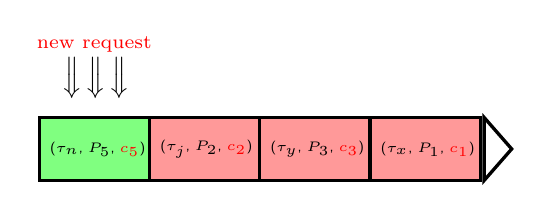
\begin{tikzpicture}[
  every node/.append style={transform shape},
  queuesty/.style={fill=white, very thick, font=\tiny},
  queuestyRed/.style={fill=red!40, very thick, font=\tiny},
  queuestyGreen/.style={fill=green!50, very thick, font=\tiny},
  srpsty/.style={fill=white, draw, circle, text width=.17cm, font=\tiny, very thick},
  numsty/.style={text width=.1cm, font=\tiny},
  arrow/.style={->},
  length/.style={red, |-|, line width=1.5pt},
  littletext/.style={font=\sffamily\tiny,inner sep=0pt,outer sep=-2pt,fill=white},
  ressty/.style={fill=red!30, draw, very thick, rounded corners=5pt},
  empty/.style={rectangle, minimum width=.7cm,font=\footnotesize}]

\begin{scope}
\draw[queuestyGreen] (0,0) node[right,yshift=0.4cm]{\sffamily ($\tau_n$, $P_5$, {\color{red}$c_5$})} rectangle +(1.4,0.8);
\draw[queuestyRed] (1.4,0) node[right,yshift=0.4cm]{\sffamily ($\tau_j$, $P_2$, {\color{red}$c_2$})} rectangle +(1.4,0.8);
\draw[queuestyRed] (2.8,0) node[right,yshift=0.4cm]{\sffamily ($\tau_y$, $P_3$, {\color{red}$c_3$})} rectangle +(1.4,0.8);
\draw[queuestyRed] (4.2,0) node[right,yshift=0.4cm]{\sffamily ($\tau_x$, $P_1$, {\color{red}$c_1$})} rectangle +(1.4,0.8);
\draw[queuesty] (5.65,0) -- (5.65,0.8) -- (6,0.4) -- cycle;

\path(0.2, 1.3)node[above,rotate=270] {${\Longrightarrow}$};
\path(0.5, 1.3)node[above,rotate=270] {${\Longrightarrow}$};
\path(0.8, 1.3)node[above,rotate=270] {${\Longrightarrow}$};
\path(0.5, 1.5)node[above,xshift=0.2cm,font=\scriptsize] {\color{red} new request};

% \draw[arrow,dashed,red,thin] (7.6,1.3) to[out=180,in=90] (4.9, 0.9);

\end{scope}

% \begin{scope} [xshift=8cm]
%   \mrspRedCeiling
% \end{scope}

\end{tikzpicture}}

\newcommand{\queueFourth}{
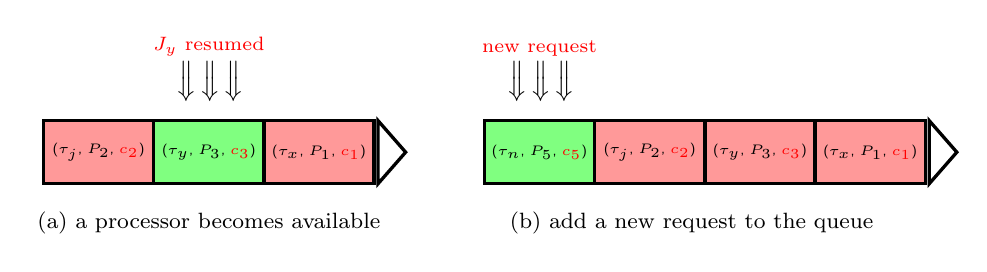
\begin{tikzpicture}[
  every node/.append style={transform shape},
  queuesty/.style={fill=white, very thick, font=\tiny},
  queuestyRed/.style={fill=red!40, very thick, font=\tiny},
  queuestyGreen/.style={fill=green!50, very thick, font=\tiny},
  srpsty/.style={fill=white, draw, circle, text width=.17cm, font=\tiny, very thick},
  numsty/.style={text width=.1cm, font=\tiny},
  arrow/.style={->},
  length/.style={red, |-|, line width=1.5pt},
  littletext/.style={font=\sffamily\tiny,inner sep=0pt,outer sep=-2pt,fill=white},
  ressty/.style={fill=red!30, draw, very thick, rounded corners=5pt},
  empty/.style={rectangle, minimum width=.7cm,font=\footnotesize}]

\begin{scope}
\draw[queuestyRed] (1.4,0)   rectangle +(1.4,0.8) node[midway]{\sffamily ($\tau_j$, $P_2$, {\color{red}$c_2$})};
\draw[queuestyGreen] (2.8,0) rectangle +(1.4,0.8) node[midway]{\sffamily ($\tau_y$, $P_3$, {\color{red}$c_3$})};
\draw[queuestyRed] (4.2,0)   rectangle +(1.4,0.8) node[midway]{\sffamily ($\tau_x$, $P_1$, {\color{red}$c_1$})};
\draw[queuesty] (5.65,0) -- (5.65,0.8) -- (6,0.4) -- cycle;

\path(3, 1.3)node[above,rotate=270] {${\Longrightarrow}$};
\path(3.3, 1.3)node[above,rotate=270] {${\Longrightarrow}$};
\path(3.6, 1.3)node[above,rotate=270] {${\Longrightarrow}$};
\path(3.3, 1.5)node[above,xshift=0.2cm,font=\scriptsize] {\color{red} $J_y$ resumed};

\path(1.2, -0.5)node[right] {{\footnotesize (a) a processor becomes available}};

% \draw[arrow,dashed,red,thin] (7.6,1.3) to[out=180,in=90] (4.9, 0.9);

\end{scope}

\begin{scope}[xshift=7cm]
\draw[queuestyGreen] (0,0) rectangle +(1.4,0.8) node[midway]{\sffamily ($\tau_n$, $P_5$, {\color{red}$c_5$})};
\draw[queuestyRed] (1.4,0) rectangle +(1.4,0.8) node[midway]{\sffamily ($\tau_j$, $P_2$, {\color{red}$c_2$})};
\draw[queuestyRed] (2.8,0) rectangle +(1.4,0.8) node[midway]{\sffamily ($\tau_y$, $P_3$, {\color{red}$c_3$})};
\draw[queuestyRed] (4.2,0) rectangle +(1.4,0.8) node[midway]{\sffamily ($\tau_x$, $P_1$, {\color{red}$c_1$})};
\draw[queuesty] (5.65,0) -- (5.65,0.8) -- (6,0.4) -- cycle;

\path(0.2, 1.3)node[above,rotate=270] {${\Longrightarrow}$};
\path(0.5, 1.3)node[above,rotate=270] {${\Longrightarrow}$};
\path(0.8, 1.3)node[above,rotate=270] {${\Longrightarrow}$};
\path(0.5, 1.5)node[above,xshift=0.2cm,font=\scriptsize] {\color{red} new request};

\path(0.2, -0.5)node[right] {{\footnotesize (b) add a new request to the queue}};

% \draw[arrow,dashed,red,thin] (7.6,1.3) to[out=180,in=90] (4.9, 0.9);

\end{scope}

% \begin{scope} [xshift=8cm]
%   \mrspRedCeiling
% \end{scope}

\end{tikzpicture}}

\section{Implementation}

% \begin{frame}

% 	\frametitle{Implementation}
% 	\framesubtitle{Development environment}

% 	The LITMUS\textsuperscript{RT} is a real-time extension of the Linux kernel.

% 	\vspace{0.3cm}
	
% 	It provides the following fundamental features:

% 	\begin{itemize}
% 		\item add a class at the top of the scheduling classes' hierarchy;
% 		\item simple plugin interface for implementing of scheduling and resource access algorithms;
% 		\item real-time domain abstraction.
% 	\end{itemize}

% \end{frame}

\begin{frame}

	\frametitle{Implementation}
	\framesubtitle{Data structures}

	\centerline{\system{1}{1}}

\end{frame}

\begin{frame}

	\frametitle{Implementation}
	\framesubtitle{Queue management - 1}

	Focused on managing the access requests queue

	\vspace{0.2cm}

	\centerline{\queueFirst{1}{1}}

	\vspace{0.2cm}

	If preempted, the lock holder ($J_x$)
		\begin{enumerate}
			\item inherits the ceiling ($c_3 + 1$)
			\item migrates to $P_3$
			\item preempts $J_y$
		\end{enumerate}
\end{frame}

\begin{frame}

	\frametitle{Implementation}
	\framesubtitle{Queue management - 2}

	% However, if there aren't available processors, the job will be re-queued in the \emph{ready\_queue}.

	The job will be re-queued in the \emph{ready\_queue}

	\vspace{0.1cm}

	\centerline{\queueSecond{1}{1}}

	\vspace{0.1cm}

	The algorithm catches the operations that 

\begin{figure}[htb]
	\centering
		\begin{subfigure}[b]{0.99\textwidth}
			\centering
			\resizebox{\linewidth}{!}\queueFourth
		\end{subfigure}
 \end{figure}
  
	% \begin{itemize}
	% 	\item add a new request to the queue
	% 	\item when a processor becomes available
	% \end{itemize}

\end{frame}

\begin{frame}

	\frametitle{Implementation}
	\framesubtitle{Primitive: mrsp\_lock}

	\begin{figure}
		\includegraphics[width=\linewidth]{../images/slides/slide_mrsp_lock.png}
	\end{figure}

\end{frame}

\begin{frame}

	\frametitle{Implementation}
	\framesubtitle{Primitive: mrsp\_unlock}

	\begin{figure}
		\includegraphics[height=7cm]{../images/slides/slide_mrsp_unlock.png}
	\end{figure}

\end{frame}

% \begin{frame}

% 	\frametitle{Implementation}
% 	\framesubtitle{Primitive: pfp\_schedule and finish\_switch}

% 	In the schedule primitive:

% 	\begin{itemize}
% 		\item a job can execute only if its priority is higher than the local ceiling;
%  		\item if preempted, the lock holder is marked for migration. 
%  	\end{itemize}

%  	After a context switch:

% 	\begin{itemize}
% 		\item the migrations take place
% 		\begin{itemize}
% 			\item the job inherites the ceiling value + 2
% 			\item it is queued in the ready\_queue;
% 		\end{itemize}
%  		\item when a waiting job resumes execution, if the lock holder has been preempted, the protocol would yield the processor to it.
%  	\end{itemize}

% \end{frame}

\begin{frame}
	\frametitle{Implementation}
	\framesubtitle{Primitive: pfp\_schedule and finish\_switch - 1}

	\centerline{\MrsPProtocolsHarder}

	\begin{itemize}
	\item $t_1$: $J_2$ is marked for migration
	\item $t_2$: $J_4$'s priority is lower than the local ceiling
	\item $t_3$: default migration mechanism
	\end{itemize}
\end{frame}

\begin{frame}
	\frametitle{Implementation}
	\framesubtitle{Primitive: pfp\_schedule and finish\_switch - 2}

	\centerline{\MrsPProtocolsHarderBis}

	\begin{itemize}
	\item $t$: $J_1$ completes and $P_1$ returns available
	\end{itemize}
\end{frame}
